\section{Bjorken/Milne Coordinates}
\label{Bjorken_Coordinates}
\footnote{\textcolor{red}{what Margaret calls them on page 12}}
In this system, two familiar quantities are used as the first two coordinates: proper time, $\tau$ \textcolor{red}{of an object with $\mathbf{x}_\perp=0$? which set off from the origin with constant velocity?} -- which is invariant under boosts along the longitudinal direction, ($x^1$) --, and rapidity \textcolor{red}{of some body in some particular circumstances too}, $\eta$. The transverse coordinates are unchanged, as in light-cone coordinates.
\begin{equation}
\begin{split}
	\tau & = \sqrt{(x^0)^2 - (x^1)^2} = \sqrt{2x^+ x^-} \\
	\eta & = \frac{1}{2} \log \left( \frac{x^0+x^1}{x^0-x^1} \right) = \frac{1}{2} \log \left(\frac{x^+}{x^-} \right)
\end{split}
\end{equation}

As for the inverse transformation,
\begin{equation}
	x^+  = \frac{\tau}{\sqrt{2}} e^\eta \qquad
	x^-  = \frac{\tau}{\sqrt{2}} e^{-\eta}
\end{equation}

\begin{figure}[H]
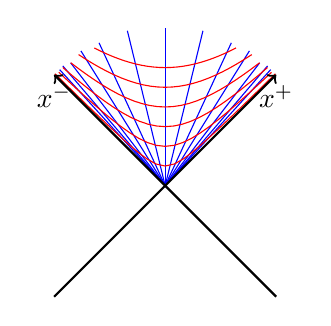
\begin{tikzpicture}
%\eta rapidity
\draw[color=blue] (0,0) -- (0,2); %0
\draw[color=blue][domain=-0.48:0.48] plot (\x,{4.1*abs(\x)}); %0.25
\draw[color=blue][domain=-0.84:0.84] plot (\x,{2.16*abs(\x)}); %0.5
\draw[color=blue][domain=-1.07:1.07] plot (\x,{1.6*abs(\x)}); %0.75
\draw[color=blue][domain=-1.2:1.2] plot (\x,{1.3*abs(\x)}); %1
\draw[color=blue][domain=-1.3:1.3] plot (\x,{1.17*abs(\x)}); %1.25 
\draw[color=blue][domain=-1.34:1.34] plot (\x,{1.1*abs(\x)}); %1.5
%\tau proper times
\draw[color=red][domain=-1.4:1.4] plot (\x,{sqrt(\x*\x+0.0625)}); %0.25
\draw[color=red][domain=-1.35:1.35] plot (\x,{sqrt(\x*\x+0.25)}); %0.5
\draw[color=red][domain=-1.3:1.3] plot (\x,{sqrt(\x*\x+0.563)}); %0.75
\draw[color=red][domain=-1.2:1.2] plot (\x,{sqrt(\x*\x+1)}); %1
\draw[color=red][domain=-1.1:1.1] plot (\x,{sqrt(\x*\x+1.563)}); %1.25
\draw[color=red][domain=-0.9:0.9] plot (\x,{sqrt(\x*\x+2.25)}); %1.5
%axes
\draw[->,thick] (1.41,-1.41) -- (-1.41,1.41) node[below] {$x^-$};
\draw[->,thick] (-1.41,-1.41) -- (1.41,1.41) node[below] {$x^+$};
\end{tikzpicture}
\centering
\caption{Contour lines for proper time, $\tau$, in red, and rapidity, $\eta$, in blue, in the first quadrant. }
\label{fig:bjorken_coordinates}
\end{figure}

We may find the new basis vectors: \textcolor{red}{versores n deviam ser "e"}
\begin{equation*}
	\vec{r} =  x^+ \vec{e}_+ + x^- \vec{e}_-
\end{equation*}
\begin{equation}
\begin{split}
	\vec{e}_\tau & = \frac{\partial \vec{r}}{\partial \tau} = \frac{e^\eta}{\sqrt{2}} \vec{e}_+ + \frac{e^{-\eta}}{\sqrt{2}} \vec{e}_- = \frac{x^+}{\tau} \vec{e}_+ + \frac{x^-}{\tau} \vec{e}_- \\
	\vec{e}_\eta & = \frac{\partial \vec{r}}{\partial \eta} = \frac{\tau}{\sqrt{2}} e^\eta \vec{e}_+ - \frac{\tau}{\sqrt{2}}e^{-\eta} \vec{e}_- = x^+ \vec{e}_+ - x^- \vec{e}_-
\end{split}
\end{equation}
\noindent which are not, in general, of unit length.

By requiring
\begin{equation*}
	\vec{A} = A^+ \vec{e}_+ + A^- \vec{e}_- \equiv A^\tau \vec{e}_\tau + A^\eta \vec{e}_\eta, 
\end{equation*}
\noindent then
\begin{equation}
\begin{split}
	A^\tau & = \frac{x^- A^+ + x^+ A^-}{\tau} \\
	A^\eta & = \frac{x^- A^+ - x^+ A^-}{\tau^2}
\end{split}
\end{equation} 

Particularly,
\begin{equation}
	\vec{r} = \tau \vec{e}_\tau
\end{equation}

